\documentclass[12pt]{paper}
\usepackage[utf8]{inputenc}
\usepackage[T1]{fontenc}
\usepackage{fancyhdr}
\usepackage{mathrsfs}
\usepackage{amssymb}
\usepackage{tikz}
\usetikzlibrary{automata,arrows,positioning}
\usepackage{textcomp}

\pagenumbering{arabic}
\pagestyle{fancy}
\rhead{Natural Language Processing}
\renewcommand{\footrulewidth}{1pt}
\renewcommand{\arraystretch}{0.6}

\begin{document}
\title{Grundlagen zu Natural Language Processing und Analyse von GATE als NLP-Tool}
\author{Aaron Schul, Felix Ritter}
\subtitle{Projektarbeit, Bearbeitungszeitraum Sommersemester 2018\\
Fachhochschule Dortmund \\
Fachbereich 4, Informatik}
\date{\today}
\maketitle

\newpage
\tableofcontents
\newpage
\listoftables

\newpage
\section{Einleitung}
Mit voranschreitender Globalisierung und immer größeren Mengen an übertragenen Informationen steigt auch die Menge an zu verarbeitender natürlicher Sprache. Während dies bisher manuell durch den Menschen geschah, kommt allmählich aufgrund der schieren Menge von Daten vor allem im unternehmerischen Kontext und im Internet die Notwendigkeit auf, die natürliche Sprache automatisiert durch Computer verarbeiten zu lassen.

Dies bezeichnet man als Natural Language Processing (kurz NLP). Es hilft dabei, Texte beispielsweise nach Schlagworten zu durchsuchen, strukturell zu analysieren, Muster zu erkennen und teilweise sogar die Bedeutung von Geschriebenem zu verstehen und diese Semantiken darzustellen.

Mit dem Aufkommen von NLP steigt auch das Interesse an NLP-Tools, also an Programmen, welche in der Lage sind, die für NLP notwendigen Funktionalitäten übersichtlich und praktikabel bereitzustellen. Eines der bekanntesten NLP-Tools ist das von der University Of Stanford entwickelte GATE, welches eine Vielzahl von Anwendungsbereichen im NLP abdeckt.

Das Ziel dieser Arbeit ist es, eine Anforderungsanalyse für solche Tools durchzuführen und diese dann mit dem GATE-Tool abzugleichen. Somit bietet sich die Möglichkeit GATE zu analysieren und daraufhin kriterienbasiert zu evaluieren. Funktionale wie nicht-funktionale Anforderungen werden definiert.

Zu diesem Zweck werden zunächst ausführlich die Grundlagen zu NLP und dessen Tools erläutert. Die Teilschritte der Textverarbeitung werden theoretisch wie praktisch anhand von Implementierungsbeispielen erläutert. Daraufhin können mit Hilfe von Use Cases Anforderungen an diese Tools erhoben werden, auf denen Analyse und Evaluation des GATE-Tools beruhen sollen. Abgeschlossen wird die Arbeit von einer kurzen Zusammenfassung der gewonnenen Erkenntnisse, gefolgt von einem Ausblick auf mögliche zukünftige Arbeiten und Entwicklungen für NLP-relevante Domänen. 
\newpage
\section{Grundlagen von Natural Language Processing}
\subsection{Einführung}
\section{Einführung}
Der folgende Abschnitt befasst sich mit den Grundlagen zu Natural Language Processing (im Folgenden kurz NLP). Dazu gehört neben dessen Herkunft bzw. Motivation eine inhaltliche Wissensgrundlage, welche für den weiteren Verlauf der Ausarbeitung relevant ist. 

\subsubsection{Motivation und Herkunft}
\subsection{Motivation und Herkunft}
Ein Großteil der menschlichen Kommunikation findet durch natürliche Sprache statt. QUELLE Dies ist bereits seit Jahrtausenden so, jedoch hat sich die Übertragung dieser Sprache mit der Zeit verändert und weiterentwickelt. 

Damals lediglich von Mund zu Mund übertragen war der erste große Schritt die Entwicklung der Schrift. Mithilfe von Hieroglyphen, Alphabeten oder anderen Zeichen war man in nun in der Lage, natürliche Sprache über lange Zeit und/oder weite Strecken zu vermitteln. Dies erwies sich als sehr Vorteilhaft und so setzte sich die Entwicklung fort, bis man über das Morsen und das Telefon schließlich die elektronische Nachricht erfand. 
Im Rahmen der voranschreitenden Digitalisierung und Globalsierung steigt die Menge an übertragener natürlicher Sprache nach wie vor rasant an, sodass heutzutage ein Leben ohne beispielsweise die E-Mail unvorstellbar scheint (OBJEKTIVER: sodass heute etwa E-Mails einen wesentlichen Bestandteil der Kommunikation ausmachen.) . Obgleich die Übertragung durch kabelgebundene oder drahtlose Kommunikation weitgehend automatisiert ist, erfolgt die Auswertung des Inhalts größtenteils manuell durch menschliche Empfänger.

Die Daten selbst sind jedoch inzwischen kaum noch nur durch den Menschen effizient zu verarbeiten, sodass man nach einer neuen Möglichkeit sucht, dem Menschen diese Arbeit zu erleichtern, oder sogar abzunehmen. Mit diese Aufgabe beschäftigt sich NLP. 

\subsection{Hypothese}

\subsection{Methodik}

\subsection{Aufbau der Arbeit}

\section{Natural Language Processing}
\subsection{Grundlagen und thematische Einordnung}
Der folgende Abschnitt befasst sich mit den Grundlagen zu Natural Language Processing (im Folgenden kurz NLP). Dazu gehört neben dessen Herkunft bzw. Motivation eine inhaltliche Wissensgrundlage, welche für den weiteren Verlauf der Ausarbeitung relevant ist. 

\subsubsection{Definition}
NLP ist grob definiert als die automatische oder halb-automatische Verarbeitung von natürlicher Sprache. (QUELLE) Manche schließen aus dieser Definition die Erfassung der Sprache aus, da diese nicht Teil der eigentlichen Verarbeitung ist. (Der Einfachheit halber wird im weiteren Verlauf davon ausgegangen, dass die Sprache als digitale Textdatei vorliegt, wenn nicht explizit anders angegeben. Es kann sich jedoch auch um gesprochenes Wort oder Gesten handeln)

NLP überschneitet sich mit vielen wichtigen Bereichen der Wissenschaft. Hauptsächlich sind dies Linguistik und Informatik, allerdings fließen auch Psychologie, Philosopie und Mathematik bzw. Logik stark mit ein. 

\subsubsection{Ziel und funktionale Einordnung}
Das Ziel von NLP ist die Extraktion von Informationen aus gegebenen Texten, also aus einem natürlichsprachigen Input einen Wissensoutput über den Inhalt des Dokuments zu generieren. Dies wird mithilfe von NLP-Tools wie GATE umgesetzt.

Dazu ist, wie im nächsten Abschnitt beschrieben, die linguistische Analyse der Sprachstruktur der Dokumente in Teilschritten erforderlich. Auf Basis der syntaktischen Analyse kann dann eine semantische Analyse durch Einsatz sogenannter Ontologien (Sammlung von Wissen aus einer Domäne) erfolgen. Letztendlich kann somit tatsächlich Wissen über die Bedeutung aus dem Dokumenteninhalt gewonnen werden.

\subsubsection{Beispiele früher Entwicklungen}
Die Forschungsergebnisse des Linguisten Noam Chomsky seit den 1950er Jahren haben aufgezeigt, dass es grundsätzlich möglich ist, einge Aspekte der Regeln englischer Sprache zu formalisieren. In Kombination von beispielsweise Automaten und generativen Grammatiken (Abschnitt 2.4 und 2.6), die auch \textit{Chomsky-Hierarchie} genannt wird, wird verdeutlicht, wie diese automatisiert aufgefasst und nachvollzogen werden kann. Siehe dazu auch \cite{cho57}. Chomsky schaffte damit zum großen Teil die Grundlagen der Modelle heutiger Sprachanalyse-Tools.

Bereits in den 1960er Jahren versuchte man durch Sprachcomputer bzw. Chatbots wie \textit{ELIZA} (Weizenbaum 1966) die Mensch-Maschine-Kommunikation umzusetzen, indem die Textnachricht eines Benutzers automatisch durch einen Computer verarbeitet und eine plausible Antwort gegeben wurde, damals jedoch noch ohne echte Wissensbasis. Aus heutiger Sicht kann man ELIZA somit keine Möglichkeit zur "intelligenten" Kommunikation attestieren, da scheinbar der Sinn hinter den Nutzereingaben nicht gänzlich erfasst wird.

Heutige Entwicklungen im Bereich Sprachassistenzsysteme sind alltäglicher Begleiter jedes Smartphone-Nutzers geworden; sie analysieren die Spracheingaben mithilfe von NLP-Techniken bezüglich ihrer Bedeutung in Echtzeit über Clouds. (QUELLE)

\subsubsection{NLP als Annäherung an natürlichsprachliche Probleme}
Bereits bei der Mensch-Mensch-Kommunikation sind  Verständigungsprobleme vorhandenen und treten unwillkürlich auf. Die Intention einer Aussage ist etwa nicht nur abhängig von dem, was tatsächlich gesagt wird, sondern auch etwa von Gestik, Mimik und der Situation, in der kommuniziert wird. Bei der Untersuchung von geschriebenem Text in natürlicher Sprache treten diese Betrachtungen jedoch in den Hintergrund, da der Inhalt im Vordergrund steht und mitunter die Situation des Autoren unklar oder irrelevant ist. Wissen aus der Domäne ist jedoch zwingend für das Verständnis spezifischer Fachbegriffe von Nöten, daher müssen auch automatische NLP-Tools diese einbeziehen können. Zudem gibt es oft Veränderungen der Bedeutung von Sprache die stark kontextabhängig sind, wie zum Beispiel Sarkasmus oder Ironie. Auch verändern Worte im Laufe der Zeit ihre Bedeutung oder durch Rechtschreibreformen ihr Aussehen. Hier soll nicht weiter auf Aspekte der Kommunikationswissenschaften eingegangen werden, jedoch ist beispielsweise die Ambiguität einer Aussage ganz alltäglich und hat gleichsam verschiedene Auswirkungen. Solche Mehrdeutigkeiten werden durch syntaktische und semantische Fehlinterpretationen verursacht. (QUELLE)

Wo sich Menschen dabei im Zweifel auf Erfahrungen und spezifische Fachkenntnisse verlassen oder bei ihrem Kommunikationspartner nachfragen können, müssen sich Computer allein auf die vorliegenden Dokumente in Schriftform verlassen; sie wissen nichts über den Kontext des Dokuments. Wie später gezeigt wird, kann jedoch etwa Fachwissen durch domänenspezifische Wissensbasen (ABSCHNITT?) simuliert werden. 

Die Frage nach einer intelligenten, algorithmen- und / oder wissensbasierten Auswertung durch Computer stellt sich im Angesicht der aufgezeigten Besonderheiten natürlicher Sprache. Es gilt also, für NLP nicht nur die Probleme zu lösen, die generell mit präziser Automatisierung verbunden sind, sondern zusätzlich so zuverlässig wie möglich die oben genannten und der Sprache inhärenten Komplikationen zu bewältigen. 
Bereits einfache Anfragen können computergestützte Frage-Antwort-Systeme wie SQL-Datenbanken an ihre Grenzen bringen, wie die verschiedenen Formen von Mehrdeutigkeit zeigen können:

Schon das Wort \textit{überblicken} kann das Übersehen von etwas, ebenso wie das im Blick haben (Gegenteil) bedeuten.

Der Satz \textit{"Die Betrachtung des Studenten"} kann etwa als Student, der (etwas) betrachtet, oder als ein Student, der (von jemand anderem) betrachtet wird, verstanden werden. Sätze mit solch einem Satzbau (bestehend aus nominalisiertem Verb, Bezugswort und Substantiv) verursachen unwillkürlich zwei mögliche Deutungen aufgrund der unklaren Syntax.

Die Frage \textit{"Verkaufen Sie Handys und Computer von Samsung?"} kann als Frage nach allgemeinen Handys und nur Computern, spezifisch von Samsung oder nach Handys und Computern gleichermaßen nur von Samsung verstanden werden. Auch hier entsteht Unklarheit durch zwei mögliche Bezüge des einschränkenden Relativsatzes. Ob eine Aufzählung oder ein Unterschied (zwischen \textit{von Samsung} und \textit{nicht von Samsung} gemacht wird, ist syntaktisch unklar.)

\textit{"Wie schnell ist der Bus?"} und \textit{"Wie schnell ist der Bus da?"} mögen zunächst ähnlich aussehen, fragen jedoch unterschiedlichen Inhalt ab und haben nichts miteinander zu tun. Außerdem könnte der zweite Satz kontextabhängig etwa nach der Fahrzeit bis zum Ziel oder nach der Ankunftszeit, an der man einsteigen kann, fragen. Die vage Formulierung von Sätzen stellt bei der Frage nach deren Bedeutung eine Herausforderung dar, durch Untersuchung des Kontextes der Frage kann hier jedoch meist recht treffsicher geantwortet werden.

Abgesehen von diesen syntaktischen Uneindeutigkeiten muss NLP auch Hürden der inhaltlichen Mehrdeutigkeit bzw. Semantik bewältigen. Aktuell beschäftigt man sich zum Beispiel mit der Aufgabe zu erkennen, ob ein Kommentar zu einem Video der Webseite \textit{Youtube} eher positiv oder eher negativ gesinnt ist. Was hier für den Menschen schon beim ersten Lesen sofort erkennbar wird, stellt für den Computer ein ernstzunehmendes Problem dar. Tonalität und Stimmung des Kommentars, der unter einem Video als Reaktion entsteht, sind mitunter nicht direkt aus dem audiovisuellen Eindruck aus dem Video ersichtlich. (?)
Solche scheinabr simplen Probleme sind für den Menschen recht einfach zu lösen. Wie oben erwähnt existiert NLP bereits seit ca. Mitte des 20. Jahrhunderts, jedoch ist die Behandlung natürlichsprachlicher Probleme auch heute noch problematisch in der Implementierung. Wenn Systeme die oben genannte Beispiele nicht explizit ausschließen, muss die Verarbeitungslogik besondere Rücksicht auf Uneindeutigkeiten nehmen.

\subsection{Konzepte aus der Logik für NLP-Anwendungen}
Hier vllt was zu $\varepsilon$T Logik

\subsection{Linguistische Analyse}
Der folgende Abschnitt beschäftigt sich mit der Analyse der sprachlichen Struktur eines Dokumentes. Am Anfang von NLP steht die linguistische Analyse des Textes etwa bezüglich Satzstruktur und Differenzierung von Wörtern aus der Sprache und Eigennamen. Das Ziel ist die sogenannte \textit{Annotation} der Textbausteine bezüglich ihrer Bedeutung. Sachzusammenhänge und Relationen von Wörtern sollen dargestellt werden. (?)
Der folgende Abschnitt beschäftigt sich mit der Analyse der sprachlichen Struktur eines Dokumentes. Am Anfang von NLP steht die linguistische Analyse des Textes etwa bezüglich Satzstruktur und Differenzierung von Wörtern aus der Sprache und Eigennamen. Das Ziel ist die sogenannte \textit{Annotation} der Textbausteine bezüglich ihrer Bedeutung. Übergreifende Sachzusammenhänge anhand der Relationen von Wörtern sollen dargestellt werden. Textstellen, die thematisch zueinander passen, sind im Ergebnis der Analyse so annotiert. (?)

NLP kann, wie später in dieser Arbeit beschrieben, als Zusammenfassung von 6 wesentlichen Teilbereichen verstanden werden. Begonnen bei der einfachen Wortanalyse, werden später Bedeutungen und Verknüpfungen der Aussage aus Sätzen oder Wörtern auf die reale Welt analysiert. Die Linguistik befasst sich seit jeher mit der Untersuchung von natürlicher Sprache im Hinblick auf die dahinter liegenden Konstrukte. Die folgenden Teilbereiche, die daraus bekannt sind, sind bei der natürlichsprachigen Analyse identifiziert worden:
NLP kann, wie später in dieser Arbeit beschrieben, als Umsetzung vierer wesentlicher Teilbereichen aus der Linguistik verstanden werden. Begonnen bei der einfachen Wortanalyse, werden später Bedeutungen und Verknüpfungen der Aussage aus Sätzen oder Wörtern auf die reale Welt analysiert. Die Linguistik befasst sich seit jeher mit der Untersuchung von natürlicher Sprache im Hinblick auf die dahinter liegenden Konstrukte. Die folgenden Teilbereiche, die daraus bekannt sind, sind bei der natürlichsprachigen Analyse identifiziert worden:

\begin{enumerate}
\item
Morphologische Analyse - Die Zerlegung von Wörtern bezüglich ihrer Struktur. Die Komposition aus Präfix, Wortstamm und Suffix von Wörtern wird erkannt, um Fall, Tempus, Numerus etc. des Wortes zu bestimmen. Im Englischen zeigt so die Endung -ed bei Verben die Vergangenheitsform an. Dabei ist zu beachten, dass Mehrdeutigkeiten entstehen können.
\item
Syntax - Aufbau von Sätzen durch einzelne Wörter. Jede Sprache besitzt syntaktische Regelungen bezüglich der auftauchenden Wörter; im Deutschen folgt etwa auf einen Artikel irgendwann ein Substantiv oder bestimmte Signalwörter geben Satztyp und Tempus an. Auf Basis dieses Wissens können formale und strukturelle Analysen der Textbestandteile erfolgen.
\item
Semantiken - Die Identifikation der Bedeutung von einzelnen Sätzen und Wörtern. Die Semantik eines Textabschnittes wird häufig als "Logik" bezeichnet und fragt nach dessen Bedeutung bzw. Thema. Semantische Deutungen können anhand von Kompositionen einzelner Wörter und Sätzen auf Basis der semantischen Analyse erkannt werden.
\item
Kontext - Darstellung von Sachzusammenhängen aus der Vereinigung von ähnlichen Bedeutungen. Textbausteine, die sich mit dem gleichen Thema beschäftigen, werden dem gleichen Sachzusammenhang zugeordnet und als Teil dessen annotiert.
\end{enumerate}

NLP spaltet bei der Analyse diese Sprachbestandteile aus der Linguistik weiter in Teilbereiche auf.
NLP spaltet bei der Analyse diese Sprachbestandteile aus der Linguistik weiter in Teilbereiche auf und ordnet diese Aufgaben in der Implementierung Programmbausteinen zu.

\subsubsection{Allgemeine NLP Architektur}
Die Verarbeitung eines Dokumentes mittels NLP erfolgt nacheinander in einzelnen Schritten, die jeweils einen Bereich oder Teilbereich der Linguistik des Textes abbilden. Die Analyse erfolgt dabei nacheinander und wird immer feingranularer, begonnen bei einfachen grammatikalischen Analysen bis hin zu komplexen Wissensbasierten verfahren. Die folgenden Schritte stellen laut \cite{cop04} eine typische komponentenweise Architektur dar. Es ist anzumerken, dass auch mehrere Schritte gemeinsam in einem Schritt durchgeführt oder gar ganz entfallen können, abhängig von der Umsetzung anderer Stufen:

\begin{enumerate}
\item
Input Processing - Erkennung der Dokumentensprache und Normalisierung des Textes. Im ersten Schritt geht es um das korrekte Format des Eingabedokumentes für die Verarbeitung. Dieser Vorgang stellt jedoch noch keine Analyse dar, sondern dient lediglich der Vorbereitung.
\item
Morphologische Analyse - Die meisten Sprachen sind im Bezug auf ihre Grammatik und syntaktische Struktur der Wörter in Systemen abgeschlossen, etwa durch Modellierung mittels Automaten zur Erzeugung der Worte. Auch können Vokabeln in Wörterbüchern/Lexika gesammelt und Regeln auf ihnen formuliert und gespeichert werden.
\item
Part-of-Speech-Tagging - Die einzelnen Wörter eines Satzes werden im Hinblick auf den Sach- oder Satzzusammenhang, wie auch auf die Stellung der Stellung im Satz hin analysiert. Basierend auf Kontext und/oder Erfahrungswerten bzw. Heuristiken können die Wörter korrekt erfasst und deren Fall getaggt werden. Subjekte, Prädikate usw. werden identifiziert. Dazu ist eine Wissensbasis mit Trainingsdaten und die Einordnung des Kontextes darin von Nöten.
\item
Parsing - Die Ergebnisse der  der vorherigen Schritte werden weiter verarbeitet und in ein standardisiertes Format gebracht. Syntaktische Zusammenhänge, wie etwa das Zusammenfassen von Wörtern zu einer gemeinsamen Bedeutungsphrase und das Zuordnen von Verben zu einem Nomen können nach dem Parsing dargestellt werden.
\item
Disambiguation - Die Entfernung von Mehrdeutigkeiten auf Basis der Ergebnisse des Parsings stellt einen entscheidenden Schritt für die semantischen Analysen dar. Nur wenn die Aussage und der Kontext eines Satzes klar erkennbar sind, kann dessen Semantik gezielt abgeleitet werden.
\item
Context Module - Textbausteine, deren Interpretation semantisch auf dem Kontext anderer Sätze oder Wörtern beruhen, können erfasst werden. Bei Anaphern ist etwa das Verständnis des aktuellen Kontext abhängig von einer vorherigen Deutung.
\item
Text Planning - Die Sachzusammenhänge und Semantiken, die aus dem zugrundeliegenden Text extrahiert wurden, werden für die Darstellung im fertigen Text definiert. Es wird festgelegt, welche der Bedeutungen qualitativ übertragen und vermittelt werden sollen. Die Reihenfolge und Umfang der behandelten Themen wird geschätzt und definiert.
\item
Tactical Generation - Die Bedeutungen werden in Form konkreter Zeichenketten generiert, die die gewünschte Bedeutung enthalten. Diese Textbausteine basieren häufig direkt auf den Ergebnissen des vorherigen Parsings, da dort schon Bedeutungen zusammengefasst werden können. Der quantitative Teil des Textes wird erzeugt.
\item
Morpholigical Generation - Die erzeugten Sätze werden morphologisch an die Rahmenbedingungen der verwendeten Sprache angepasst. Grammatiken und Regeln der Satzkonstruktion werden auf die erzeugten Wörter angewendet, sodass ein lesbarer und nachvollziehbarer Text entsteht.
\item
Output Processing - Der Text wird nun, nachdem dieser inhaltlich nun komplett erzeugt vorliegt, an das Design und Format des jeweiligen Einsatzzwecks angepasst. Sollte Text, anders als in dieser Arbeit der Einfachheit halber angenommen, nicht als geschriebenes Wort ohne besondere Formatierung vorliegen, kann dieser einem Formatter zur Designanpassung übergeben werden. Ferner kann etwa mihilfe von Text-to-Speech eine Audioausgabe erfolgen. 
\end{enumerate}

\subsection{Morpholoie in NLP}
Der folgende Abschnitt befasst sich genauer mit der morphologischen Analyse von Wörtern und den dazu verwendeten Zustandswandlern. Da in der englischen Sprachanalyse bereits die meisten Fortschritte erzielt wurden und sie verhältnismäßig wenig komplex im Vergleich zu anderen Sprachen ist, werden im Folgenden viele der Beispiele auf Englisch behandelt. (? vielleicht trennen)

Wie bereits erwähnt, befasst sich die Morphologie mit der Struktur, Zusammensetzung und Korrektheit einzelner Wörter. Jedes Wort der englischen Sprache besteht aus mindestens einem Wortstamm und beliebig vielen Affixen. Affixe sind unterteilt in Präfixe und Suffixe, abhängig davon, ob sie vor oder hinter dem Wortstamm auftauchen. Es gibt auch Affixe, welche in der Mitte des Wortes eingeordnet werden. Diese existieren jedoch nicht in der englischen Sprache und sind daher künftig zu vernachlässigen. (? Reihenfolge)

Man betrachte beispielsweise das Wort \textit{"believe"} von dem englischen Verb \textit{"to believe"} (zu Deutsch: "glauben"). (kürzer) Hängt man das Suffix \textit{"-able"} an, so erhält man das Adjektiv \textit{"believable" ("glaubhaft")}. Fügt man nun das Präfix \textit{"un-"} hinzu erhält man die Negation \textit{"unbelievable" ("unglaubhaft")}. Die morphologische Analyse erkennt dies nicht nur als ein Wort, sondern als Präfix-Stamm-Suffix-Konstrukt.

Es wird zwischen ableitender und flexionaler Morphologie unterschieden, wobei die Abgrenzung jedoch nicht ganz eindeutig ist. Affixe wie \textit{"anti-"}, \textit{"re-"} und das oben verwendete \textit{"un-"} gelten als ableitend und können mehrfach und sogar rekursiv zu Stämmen auftauchen. Sie fügen dem Stamm in der Regel eine Zusatzinformation hinzu, wie z.B. Negation. Es kann auch, wie in dem Beispiel oben demonstriert, zur Änderung der Wortart kommen. Flexionale Affixe werden normalerweise aufgrund grammatikalischer Regeln wie Pluralisierung hinzugefügt. Hierzu gehören das Plural-"-s" und die Endung \textit{"-ed"} in der Vergangenheitsform. 

Die morphologische Analyse ist üblicherweise eine Vorarbeit für das Parsen von Texten, welches in Abschnitt 2.6 genauer beschrieben ist. Dafür sind jedoch genauere syntaktische und semantische Informationen nötig. So würde beispielsweise das Wort "fishing" eindeutig durch die "-ing"-Endung als Verb im Partizip Präsens erkannt, während bei dem Wort "fish" eine Mehrdeutigkeit zwischen dem Verb "fischen" und dem Substantiv "Fisch" die Verarbeitung verkompliziert. Dies wird durch das sogenannte Part-of-Speech-Tagging gelöst, welches in Abschnitt 2.5 behandelt wird.

\subsubsection{Lexika in der Morphologie}
Für eine präzise morphologische Analyse bedarf es 3 verschiedener Lexika, um mögliche Interpretationen zu speichern:

\begin{enumerate}
\item Liste von Affixen (zusammen mit den Informationen, die damit verbunden sind, z.B. Negation \tt "un-"\rm)
\item Liste von unregelmäßigen Wörtern (zusammen mit den Informationen, die damit verbunden sind, z.B. \tt "went":simple past"(to) go"\rm)
\item Liste von Wortstämmen (zusammen mit syntaktischer Kategorie, z.B. \tt "believe":verb\rm)
\end{enumerate}

Die Affix-Liste könnte in einen Präfix- und einen Suffix-Teil getrennt werden, welche jeweils das Affix und die oben beschriebenen Informationen als formatierten Text enthalten, in etwa wie folgt (Suffix-Teil):
\\
\tt
ed PAST\_VERB\\
ed PSP\_VERB\\
s PLURAL\_NOUN\\
\rm
PAST\_VERB, PSP\_VERB und PLURAL\_NOUN beinhalten die durch den jeweiligen Suffix hinzugefügten Informationen über das Wort. 

Ähnlich verhält es sich mit der Auflistung der unregelmäßigen Formen. Das Affix wird hier durch die unregelmäßige Form ersetzt und es ist zu beachten, dass es nötig ist, zu den in 1. vorhandenen Informationen auch den Referenz-Stamm anzugeben, in etwa wie folgt:
\\
\tt
began PAST\_VERB begin\\
begun PSP\_VERB begin\\
\rm
\textit{"Began"} und \textit{"begun"} sind hier jeweils die "PAST\_VERB"- und "PSP\_VERB"(past participle)-Form des Referenzstammes \textit{"begin"}.

Um unnötige Fehler zu vermeiden ist es ratsam, zusätzlich ein Lexikon mit Wortstämmen zu verwenden, welches die Wortstämme und eine grammatikalische Einordnung beinhaltet. Dies hat hauptsächlich zwei Gründe: 

\begin{enumerate}
\item Die Form im Zusammenhang mit vielen syntaktischen (siehe Abschnitt 2.5) und morphologischen Regeln ist wichtig. Die \textit{"-able"}-Anhangsregel kann beispielsweise nur bei Verben verwendet werden, die dann ein Adjektiv darstellen (diese Eigenschaft würde in der Affix-Liste beschrieben).
\item Mögliche Wortstämme überprüfen zu können ist wichtig, da somit viele Mehrdeutigkeiten ausgeschlossen werden können. So könnte "bus" z.B. als "bu$\textasciicircum$s" (Plural von "bu") interpretiert werden. Dies ist jedoch nicht möglich, wenn kein Eintrag zu dem Wortstamm "bu" existiert. 
\end{enumerate}

\subsubsection{Buchstabierregeln mit endlichen Zustandswandlern}
In der Morphologie gibt es eine Vielzahl von Regeln, die bei der Unterteilung, Interpretation und Zusammensetzung von Wörtern zu beachten sind. Wenn man das "believe"-Beispiel aus Abschnitt 2.4 erneut betrachtet, fällt auf, dass bei dem hinzufügen des Suffixes "-able" der letzte Buchstabe des Wortstammes entfällt. Dies ist natürlich kein Tippfehler, sondern beruht auf einer der besagten Regeln. Die oben verwendete Regel lässt sich wie folgt darstellen:
\tt
\begin{center}
e $\rightarrow \varepsilon \textasciicircum \_$able
\end{center}
\rm
Das \textit{e} ist in dem Falle der in Frage stehende Buchstabe, welcher, symbolisiert durch den Pfeil, in das $\varepsilon$ (das leere Wort) gewandelt wird, falls ein Affix angehängt wird ($\textasciicircum$) und es an dieser Stelle ($\_$) steht, also vor dem \textit{"-able"}.

Solche Regeln lassen sich zu morphologischen Zwecken gut mit endlichen Zustandswandlern (finite state transducers) realisieren, was im Folgenden demonstriert werden soll.

\subsubsection{Endliche Zustandswandler zur Umsetzung von morphologischen Regeln}
Ein endlicher Zustandswandler ist ein Graph aus einer endlichen Anzahl von Knoten (Zuständen), welche durch Kanten verbunden sind. Knoten sind unterteilt in einen Start-Knoten, eine beliebige Anzahl an normalen Knoten und mindestens einen Ziel-Knoten. Der Start-Knoten als Input das zu verarbeitende Wort, welches nun in eine Abbildung der Aufbaustruktur des Wortes übertragen werden soll. Das Erreichen eines Ziel-Knotens heißt, dass das Wort korrekt ist und akzeptiert werden kann. Die Kanten repräsentieren die Abbildung einer Zeichenkette auf eine andere. Dies funktioniert bidirektional, wodurch sie sowohl zum Erstellen, als auch zum Auflösen von Wörtern verwendetet werden können. Die folgende Abbildung zeigt den eindlichen Zustandswandler, der die Umsetzung der besagten "able"-Anhangs-Regel ermöglicht: (QUELLE AUTOMATEN)
\\
\\
\begin{center}
\begin{tikzpicture}

\node[accepting] (a) at (0,0)  [circle, draw, minimum size=10ex] {1};
\node (b) at (4,0)  [circle, draw, minimum size=10ex] {2};
\node (c) at (4,-4) [circle, draw, minimum size=10ex] {3};
\node[accepting] (d) at (0,-4) [circle, draw, minimum size=10ex] {4};
\draw[thick, ->] (a) to [bend left] node[midway, above] {$\varepsilon$ : e} (b);
\draw[thick, ->] (a) to [loop above] node[midway, above] {other : other} (a);
%\draw[thick, ->] (b) to [bend left] node[midway, below] {e : $\varepsilon$} (a);
\draw[thick, ->] (b) to [bend left] node[midway, right] {$\varepsilon : \textasciicircum$} (c);
\draw[thick, ->] (c) to [bend left] node[midway, below] {able:able} (d);

\end{tikzpicture}
\end{center}

Der oben abgebildete Zustandswandler ist in der Lage die beschriebene Regel umzusetzen wie folgt: In Zustand 1 erfolgt der Input des eingelesenen Wortes, also in diesem Falle \textit{"believable"}. Über die Schleife mit \textit{"other:other"} ist die Abbildung aller nicht speziell angegebenen Zeichenfolgen auf sich selbst beschrieben. Es kann jederzeit das leere Wort auf ein \textit{"e"} Übertragen werden, dies geschieht jedoch nur, falls auch ein "-able" folgt. In dem Fall wird zuvor noch aus dem leeren Wort ein Affix-Zeichen ($\textasciicircum$) generiert (Es ist anzumerken, dass der Zustandswandler nicht deterministisch ist, sich jedoch über die Potenzmengenkonstruktion immer ein äquivalenter deterministischer Zustandswandler erstellen ließe). So wird also das Wort "believable" durch diesen Automaten als "believe$\textasciicircum$able" Interpretiert, und somit das "able"-Affix erkannt. Andersherum ließe sich aus dem Wortaufbau "believe$\textasciicircum$able" das korrekte Wort "believable" generieren. (QUELLE NEA VL von PREIS?)

Üblicherweise werden für jede Regel eigene Zustandswandler erstellt, welche dann bei der Verarbeitung von Wörtern parallel ablaufen. Dies ist gut für die Performanz, birgt allerdings Probleme. Wenn man mit komplexen Wörtern arbeitet, bei denen mehrere Regeln gleichzeitig anzuwenden sind, können verschiedene valide Ergebnisse erzielt werden. So wäre es etwa problematisch zwischen den Wörtern "un$\textasciicircum$ion$\textasciicircum$ise$\textasciicircum$ed" (Chemie) und "union$\textasciicircum$ise$\textasciicircum$ed" (gewerkschaftlich organisiert) zu unterscheiden. 

\subsection{Part-of-speech tagging und Wortvorhersage}
Dieses Kapitel befasst sich mit der Transformation von Ergebnissen der morphologischen Analyse einzelner Wörter in eine sinnvolle Kategorisierung der Wörter im Sachzusammenhang aus mehreren Wörtern. Part-of-speech tagging klassifiziert einzelne Worte eines Textes so, dass erfasst wird, welche Rolle sie im Satz spielen. Die einzelnen Wörter des Textes werden im Englischen bezüglich ihrer grammatikalischen Funktion und Anzahl markiert (\textit{annotiert}). Die Identifikation muss so erfolgen, dass sie den Kontext des Satzes erfasst, also insgesamt Sinn ergibt. Diese Kennzeichnung geht über die Analyse einzelner Wörter hinaus; Sie erfasst auch die Syntax umgebender Wörter eines Satzes. 

Im Deutschen ist es etwa recht wahrscheinlich, dass auf ein Nomen am Satzanfang als nächstes Wort ein Verb folgt, da dies einen typischen Satzbau darstellt. Ein part-of-speech Tagger sollte daher beispielsweise im Satz \textit{"Ich fahre Fahrrad."} korrekt das "Ich" als Subjekt, das "fahre" als Prädikat und das "Fahrrad" als Akkusativobjekt darstellen; Die isolierte Betrachtung von \textit{"Fahrrad"} ließe aber auch die Kategorisierung als Subjekt zu, da sich die zwei Möglichkeiten bezüglich der Morphologie nicht unterscheiden. Diese Mehrdeutigkeit einzelner Worte im Satz wird durch Analyse des syntaktischen Kontextes eliminiert, sodass POS tagging eine Eindeutigkeit der syntaktischen Deutung erzielt.

Solche Regelmäßigkeiten werden in Form von sogenannten \textit{corpora} geliefert; sie stellen Trainingsdaten in Form von tatsächlicher Sprache dar. Im Englischen wird etwa häufig die Zeitung The Wall Street Journal genutzt, um die Repräsentation bestimmter Satzstrukturen und Wortfolgen statistisch zu erfassen. Alternativ können auch standardisierte Corpora wie der Lancaster-Oslo-Bergen Corpus (QUELLE) verwendet werden, der etwa eine Million Wörter in Sprache enthält. Corpora sind etwa für NLP auf Basis von Machine-Learning-Algorithmen erforderlich, können darüber hinaus aber auch etwa zur Rechtschreibprüfung oder Textunterteilung benutzt werden. Die meisten Textverarbeitungsprogramme können heutzutage etwa erkennen, wenn sich syntaktische Fehler in einem Satz ereignen (Kommasetzung, falscher Kasus, etc.). Es ist anzumerken, dass part-of-speech tagging nicht unbedingt vorher annotierter Texte bedarf, aber ohne diese eine syntaktische Einordnung ungleich schwerer fällt und die Fehlerquote massiv steigt. Mehrdeutigkeiten aus der Syntax heraus können somit nicht aufgeschlüsselt werden.

Die Anwendung eines Corpus auf ein natürlichsprachliches Dokument ermöglicht sogleich auch eine Vorhersage der nächsten Wörter bzw. Sprachbausteine, nachdem schon ein Teilsatz gelesen wurde. Diese \textit{prediction} kann auf Basis bekannter Regelmäßigkeiten also schon vor der Wortanalyse recht genau die nächste grammatikalische Komponente bzw. den Worttyp vorhersagen.

\subsubsection{N-gram Modelle zur Sprachvorhersage und -modellierung}
Auf Basis der vorliegenden Corpora existieren eine Vielzahl an Regeln bezüglich des Satzbaus und bekannnter Folgen von Worttypen, wenn ein neues Dokument annotiert werden soll. Zur Veranschaulichung einer möglichen Annotation soll in diesem Abschnitt die Notation \cite{clw7} für Annotationen genutzt werden.

Bei erneuter Betrachtung des obigen Beispiels \textit{"Ich fahre Fahrrad."} könnte dieses, wenn dieser Satz als minimaler Corpus vorliegt, neben der Regel Subjekt-Prädikat-Objekt eines Satzbaus auch beinhalten, dass der Punkt ein Satzende markiert und das Substantive und Satzanfänge mit einem Großbuchstaben beginnen ("Fahrrad" ist gemäß der Morphologie ein Nomen und ist groß geschrieben). Sprachvorhersage nutzt diese bekannten Regeln und würde etwa aus der obigen Regel herleiten, das, wenn ein Verb gelesen wurde, darauf immer ein Substantiv bzw. das Satzobjekt folgt. POS-Tagging macht sich diese Beobachtungen durch Berechnung von Wahrscheinlichkeiten bei der Annotation von Wortfolgen zunutze. 

Kontextfreie Betrachtung einzelner Wörter, also ohne andere Taggings mit einzubeziehen, wird als Unigramm bezeichnet. Dabei werden jedoch Regeln über den Zusammenhang von Wortketten vollständig ignoriert und das Ergebnis ist ähnlich dem der morphologischen Analyse. Vorhersage-Systeme, die sich der Annotierung des vorigen Wortes bedienen, werden als Bigramme (englisch \textit{bigrams}) bezeichnet, Trigramme dementsprechend bei Berücksichtigung der zwei vorigen Wörter und N-gramme, wenn alle n-1 zuvor gelesenen Wörter, also die gesamte Terminologie des Textes bis zum n-ten Wort, berücksichtigt werden.
Die Wahrscheinlichkeit des Typs des Folgewortes auf Basis eines Bigramms lässt sich berechnen, indem aus einem Corpus die Worttypen an der jeweiligen Satzstelle gezählt und statistisch erfasst werden. 
Als Beispiel dazu soll hier zunächst ein Bigramm zur tatsächlichen Wortvorhersage dienen, anschließend wird erläutert, inwiefern solche Techniken auch den nächsten part-of-speech in einem Text vorhersagen können. Aus folgendem Corpus vierer Aussagen lässt sich dies wie folgt ableiten:
\\ \tt

<s> ich mag Züge <s> ich mag guten Tee 


<s> guten Morgen <s> guten Abend <s>
\\ \rm

Zwischen einzelnen Äußerungen wird der Platzhalter <s> als Indikator einer neuen Aussage verwendet, sodass dem Bigramm nun eine Zeichenkette mit den obigen Aussagen getrennt durch \tt <s> \rm zur Verfügung steht. Nun wird die mögliche Wortkombinatorik aus dem Corpus extrahiert, indem Kombinationen gezählt werden. Berechnet werden nun die Wahrscheinlichkeiten des Folgewortes auf Basis der vorherigen, formal ausgedrückt: $\frac{C(w_{n-1} w_{n})}{\sum{w}{}C(w_{n-1}w)}$
\tt
\begin{table}[h]
\begin{tabular}{lll}
Sequenz & Anzahl & $P(w_{n}|P(w_{n-1})$ \\
<s> & 4 & \\
<s> ich & 2 & 0,50 \\
<s> guten & 2 & 0,50 \\ 
ich mag & 2 & 1,0 \\ 
mag Züge & 1 & 0,5 \\
mag guten & 1 & 0,5 \\
Züge & 1 & \\
Züge <s> & 1 & 1 \\
guten & 3 & \\
guten Tee & 1 & $\frac{1}{3}$ \\
guten Morgen & 1 & $\frac{1}{3}$ \\
guten Abend & 1 & $\frac{1}{3}$ \\
Tee & 1 & \\
Tee <s> & 1 & 1 \\
Morgen & 1 & \\
Morgen <s> & 1 & 1 \\
Abend & 1 & \\
Abend <s> & 1 & 1\\
\end{tabular}
\caption{Wahrscheinlichkeitstabelle Bigram zur Wortvorhersage}
\end{table}
\rm
Es lassen sich nun die Wahrscheinlichkeiten des jeweils nächsten Wortes nach einem gelesenen Wort ablesen. Auf "ich mag" folgt insgesamt einmal "Züge" und einmal "guten". Daher kann nun genau die Wahrscheinlichkeit des nächsten Wortes "Züge" mit $P("$Züge$"|$"ich mag"$)$ = 50\% berechnet werden.

\subsubsection{Stochastisches POS-tagging}
Neben der Möglichkeit, einzelne Wörter vorherzusagen, eignen sich n-Gramme wie oben erwähnt auch zur Darstellung der Wahrscheinlichkeiten von Satzbausteinen, also der von Platzhaltern für alle möglichen Wörter einer Kategorie bzw. Komponente. Stochastisches Part-of-speech tagging kann anhand dieser die Wahrscheinlichkeiten vorhersagen, welcher Worttyp folgen wird. Die Trainingsdaten sind, nach Best-Practices aus dem maschinellen Lernen, in der Regel manuell und durch Benutzer markiert worden, damit dem Programm ein korrekter Datensatz zur Verfügung steht. Auf Basis eines Corpus können somit Mehrdeutigkeiten durch den syntaktischen Zusammenhang eindeutig aufgelöst werden. In einem Beispiel mit syntaktischer Ambiguität werden jedoch Wörter zunächst verschieden annotiert.
Das tagset von CLAWS 7 annotiert Wortkategorien wie folgt:

\tt 
\begin{table}[h]
\begin{tabular}{ll}
PPIS2	& 1st person plural subjective personal pronoun \\
PPHO1	& 3rd person sing. objective personal pronoun\\
NN1		& singular common noun \\
VV0		& base form of lexical verb \\
VVD		& past tense of lexical verb \\
PUN		& punctuation
\end{tabular}
\caption{Annotationen gemäß \cite{clw7} (Auszug)}
\end{table} 

%NN1 Nomen im Singular. \\
%PNP Personalpronomen.\\
%VM0 Modales Hilfsverb.\\
%VVB Verb in Grundform ohne Appendix.\\
%VVI Verb im Infinitiv (im Englischen mit "to").\\
\rm

Als Beispiel dient hier der englische Satz \textit{"We saw her duck."}. Dieser enthält Mehrdeutigkeiten, da "duck" entweder als \textit{"Ente"}, also als Substantiv \textit{"ihre Ente"} oder als "ducken", also als Verb (dt. \textit{"sie (sich) ducken"}) interpretiert werden kann. Zusätzlich kann "we saw" als \textit{"sahen"}, oder als \textit{"zerschneiden"}, also zeitformabhängig verstanden werden. Äquivalent im Deutschen sind also die drei Sätze \textit{"Wir sahen ihre Ente."}, \textit{"Wir sahen sie (sich) ducken."} und \textit{"Wir zerschneiden ihre Ente"} mit völlig unterschiedlicher Aussage. (Semantisch betrachtet stellt sich ferner die Frage, ob die Deutung von "her duck" als Nomen mit "ihr Haustier" etwas anderes bedeutet als "für sie zum Essen")

Diese sinnvollen Annotationen könnten durch einen CLAWS 7-POS-tagger wie folgt erfasst werden:

\tt
\begin{tabular}{ll} 
1. & We(PPIS2) saw(VVD) her(PPHO1) duck(VV0) .(PUN) \\
2. & We(PPIS2) saw(VVD) her(PPHO1) duck(NN1) .(PUN) \\
3. & We(PPIS2) saw(VV0) her(PPHO1) duck(NN1) .(PUN) \\
\end{tabular} \rm

Problematisch ist, dass auch syntaktisch falsche Deutungen entstehen können, wenn, wie oben erwähnt, unzureichende Trainingsdaten und Regeln für die Wortfolgen existieren. Dann werden alle möglichen Teildeutungen der einzelnen Wörter als Tagging ausgegeben, etwa mit der Bedeutung \textit{"Wir zerschneiden sie sich ducken"} aus der Syntax.

\tt
\begin{tabular}{ll} 
4. & We(PPIS2) saw(VV0) her(PPHO1) duck(VV0) .(PUN)\\
\end{tabular} \rm

Durch das Verwenden von manuell erstellten Corpora kann zumindest diese eindeutig falsche Deutung der Syntax eliminiert werden, da solch ein Sprachkonstrukt in der englischen Sprache nicht auftreten kann. Das Tagging des folgenden minimalen Korpus könnte dann wieder als Eingabe für ein n-Gramm dienen, welches auf Basis der höchsten Wahrscheinlichkeit ein Wort annotiert.

\tt
People use to see a duck. Most people duck in order to avoid danger.
\rm

Der Corpus könnte annotiert sein:

\tt
We(NN2) use(JK) to(TO) see(VV0) a(AT1) duck(NN1).(PUN) Most(DAT) people(NN2) duck(VV0) in(BCL11) order(BCL12) to(BCL13) avoid(VV0) danger(NN1).
\rm

Dauraus ergibt sich unter Verwendung eines n-Grams umgangssprachlich formuliert, dass etwa in einem Satz, in welchem bereits ein Wort als Verb im Präsens getaggt wurde, ein Objekt, also ein als Nomen getaggtes Wort, folgen muss. Im ersten Satz ergibt sich dies etwa aus der Stellung des "see" als Verb vor dem "duck". Dementsprechend kann so schon die vorhin beschriebene Deutung 4. ausgeschlossen werden, da diese Regel des Satzbaus nicht vorkommt. Weitere mögliche Regelmäßigkeiten, die ein n-Gramm statistisch erfasst, wäre die Möglichkeit einer Before-Clause (BCL) nur nach einem Nomen oder die hohe Wahrscheinlichkeit eines Punktes nach einem Nomen im Singular. Auffällig ist, dass die Deutung von saw als Verb in Past Tense entfällt, da keine Regel auftritt, die ein Verb in Past-Tense vor einem Nomen enthält. Daher erfasst ein N-Gram auf Basis dieses Korpus nur Verben im Präsens korrekt (im Corpus taucht keine Deutung eines Verbs als Vergangenheitsform auf). 

Abschließend lässt sich daher sagen, dass die Trainingsdaten möglichst repräsentativ für die möglichen Konstruktionen in einer Sprache bzw. in der Anwendungsdomäne des POS-taggers sein müssen, um akkurate Ergebnisse zu erzielen. Dies betrifft sowohl die Qualität der im Corpus enthaltenen Wörter und Sätze, als auch deren Korrektheit im Hinblick auf die quantitative Repräsentation einzelner Konstrukte. Häufig anzutreffende Hauptsatz-Nebensatz-Konstruktionen müssen etwa für die Analyse eines stilistisch einfachen Textes, der zum Großteil aus solchen besteht, häufiger vorhanden sein, als kompliziert verschachtelte Kausalsätze und eingeschobene Relativsätze mit beispielsweise vielen beschreibenden Aufzählungen.  

\subsection{Parsen und Generieren mit kontextfreien Grammatiken}
Wie bereits in 2.4 angekündigt befasst sich dieser Abschnitt mit dem Parsen und Generieren von Sätzen auf Grundlage der vorhergegangenen Verarbeitungsschritte. Fokus liegt dabei auf der Auflösung von Mehrdeutigkeiten, welche nicht durch die morphologische Analyse und Part-of-Speech-Tagging bewältigt werden konnten. Dies wird anhand verschiedener kontextfreier Grammatiken genauer erläutert. 

\subsubsection{Generative Grammatik}
Der Begriff der generativen Grammatik beruht auf der Arbeit von Chomsky in den 1950er Jahren \cite{cho57}. Man versteht darunter eine formale Grammatik, welche in der Lage ist alle möglichen Sätze einer natürlichen Sprache und nur genau diese zu generieren. Hier ist anzumerken, dass man dem tatsächlichen Entwurf einer solchen Grammatik bisher nicht einmal nahe gekommen ist. Jedoch ist für Linguisten der prinzipielle Aufbau von solchen Grammatiken höchst interessant (vor allem von solchen Grammatiken, welche sich auf alle natürlichen Sprachen anwenden lassen), während sich NLP-Forscher eher mit dem Bau und der Nutzung von möglichst umfangreichen Grammatiken befassen. 

Ähnlich zu der ableitenden Morphologie versucht man hier, Zeichenketten eine interne Struktur zu verleihen, welche es ermöglicht, Informationen zu den einzelnen Bestandteilen zu extrahieren, jedoch tut man dies mit Sätzen (oder Satzteilen) anstelle von einzelnen Wörtern. Darstellen lässt sich diese Struktur beispielsweise durch Klammerung wie folgt:

((the (fisherman)) fishes)
((the (old fisherman)) fishes)

Durch das obige Beispiel wird die Bindung der einzelnen Wörter untereinander deutlich: "old" gehört eindeutig zu "fisherman" und das "the" bezieht sich im zweiten Satz auf "old fisherman" zusammen. Die Klammerung (the old) ist also auf keinen Fall möglich, da "old" mit dem "fisherman" eingeklammert ist. 

Bei zwei Grammatiken spricht man von schwacher Äquivalenz, falls sie die gleichen Zeichenketten generieren können und von starker Äquivalenz, wenn sie diese auch gleich klammern. 

Die meisten Ansätze verleihen der internen Struktur nun verschiedene Bezeichnungen, abhängig von der oben gezeigten Klammerung. Somit würde man "the fisherman" (ebenso wie "the old fisherman") im Englischen als "noun-phrase" (NP) bezeichnen. "fishes" würde (zusammen mit jeglichen Zusätzen wie "fishes very good" oder "fishes fish" als "verb-phrase" (VP) gekennzeichnet. Diese Bezeichnungen dienen in kontextfreien Grammatiken als linke Seite von Produktionsregeln, wie im folgenden Abschnitt genauer dargestellt wird.

\subsubsection{Kontextfreie Grammatiken}
Kontextfreie Grammatiken stammen aus dem Bereich der Theoretischen Informatik (QUELLE PREIS) und werden dargestellt durch ein Tupel mit 4 verschiedenen Komponenten:

\begin{enumerate}
\item Eine Menge nicht-terminaler Symbole (wie z.B. NP oder VP aus dem vorherigen Abschnitt)
\item Eine Menge terminaler Symbole (die Wörter aus denen später die Zeichenkette bestehen wird, also "the", "old", "fisherman" und "fishes")
\item Eine Menge sogenannter Produktionsregeln mit folgenden Eigenschaften:
\begin{enumerate}
\item Eine Regel besteht aus einer linken und einer rechten Seite, getrennt durch einen Pfeil ($\rightarrow$).
\item Auf der linken Seite befindet sich genau ein nicht-terminales Symbol.
\item Auf der rechten Seiten befindet sich mindestens ein Symbol (terminal oder nicht-terminal).
\end{enumerate}
\item Das Startsymbol (konventionell "S"), welches zu den nicht-terminalen Symbolen gehört
\end{enumerate}

Es ist zu beachten, dass in kontextfreien Grammatiken generell das leere Wort $\varepsilon$ als terminales Symbol mit eingeschlossen ist. Aus linguistischer Sicht verkompliziert dies jedoch nur die Grammatiken und kann daher bezüglich NLP ausgeschlossen werden (es ließe sich außerdem auch zu jeder kontextfreien Grammatik eine schwach-äquivalente Grammatik erzeugen, welche das leere Wort nicht beinhaltet).

Man spricht von einer linksbündigen bzw. rechtsbündigen Grammatik, wenn alle nicht-terminalen Symbole ganz links bzw. rechts auf der rechten Seite der Regel stehen (also in der Form "NT$\rightarrow$NT t" bzw "NT$\rightarrow$t NT"). Diese Grammatiken sind jedoch schwach-äquivalent zu regulären Grammatiken, welche sich mit endlichen Automaten implementieren lassen. Dies ist jedoch für den Aufbau von natürlichen Sprachen nicht ausreichend. Der Ansatz, sich auf eine rechts- bzw. linksbündige Grammatik zu beschränken, um damit eine natürliche Sprache zu generieren, entfällt also sofort. 

%\subsubsection{Beispiel einer kontextfreien Grammatik}
Im folgenden wird die Funktionsweise kontextfreier Grammatiken anhand eines sehr simplen Beispiels dargestellt. Hierzu gelten die folgenden Produktionsregeln P (für spätere Erläuterungen durchnummeriert):
\newline
\\
\tt
1. S $\rightarrow$ NP VP\\
2. VP $\rightarrow$ V\\
3. VP $\rightarrow$ V NP\\
4. VP $\rightarrow$ V VP\\

\rm

Außerdem stehe ein Lexikon die folgenden Wörter zur Verfügung:
\newline
\\
\tt
V $\rightarrow$ can\\
V $\rightarrow$ fish\\
V $\rightarrow$ catch\\
NP $\rightarrow$ fish\\
NP $\rightarrow$ he\\
NP $\rightarrow$ fishermen\\
\rm 
\newline
Die formale Darstellung dieser Grammatik sieht dann aus wie folgt:

\begin{center}
\tt
$G=(\lbrace S,VP,NP,\rbrace ,\lbrace can, fish, catch, he, fisherman\rbrace ,\lbrace P(siehe oben)\rbrace ,S)$
\rm
\end{center}

Man beachte, dass "fish" nur einmal bei den terminalen Symbolen auftaucht, obwohl es im Lexikon zwei mal aufgeführt ist (als verb und als noun-phrase). Diese Unterscheidung wird in der Grammatik jedoch lediglich durch die produzierende Regel vorgenommen, das terminale Symbol ist für beide Varianten zunächst gleich.

Die Möglichkeiten und Probleme der beschriebene Grammatik werden an den folgenden Beispielsätzen deutlich:
\\

\tt
"He can fish"
"He can catch fish"
"Fishermen can fish fish"
\rm

Klammert man den ersten Satz entsprechend der Grammatik kommt man zu folgendem Ergebnis:\\

\tt 
(S(NP he)(VP(V can)(VP(V fish))))\\
\rm

Somit kann man, indem man die Klammern von außen nach innen durchgeht die verwendeten Regeln und ihre Reihenfolge ermitteln, in diesem Fall also 1., 4. und dann 2.. (Dies lässt sich jedoch sehr viel übersichtlicher darstellen, wie in einem späteren Abschnitt aufgezeigt wird.)

Der gleiche Satz ließe sich aber auch leicht anders klammern:\\

\tt
(S(NP he)(VP(V can)(NP fish)))\\
\rm

Die Grammatik lässt in diesem Fall durch die 3. Produktionsregel zu, dass "fish" als noun-phrase statt verb interpretiert wird , was jedoch auf semantischer Ebene keinerlei Sinn ergibt und daher eigentlich nicht möglich sein sollte. Entfernt man die 3. Produktionsregel jedoch aus der Grammatik, so lassen sich andere, durchaus sinnvolle Sätze, wie der zweite Beispielsatz "He can catch fish" nicht mehr herstellen. Dies gilt ebenfalls für den dritten Beispielsatz "Fishermen can fish fish", welcher nur Sinn ergibt, solange "fish" als verb und als noun-phrase interpretiert werden kann.

\subsubsection{Pars-Bäume} 

Wie angekündigt lässt sich die Struktur von geparsten Sätzen auch etwas übersichtlicher darstellen. Dies geschieht mit sogenannten Pars-Bäumen

\subsubsection{Anwendung Chart-Parsing}
Wie anhand des Parsbaums zu einer zugehörigen Grammatik erkennbar ist, ist es nicht nur möglich, anhand von Produktionsregeln Sätze zu generieren, sondern diese (Teil-)Sätze aufsteigend nach den erzeugenden Regeln aufzuschlüsseln. Aus kontextfreien Grammatiken lassen sich jedoch Sätze erzeugen, die semantisch betrachtet weniger Sinn ergeben, als andere. Auch kann es passieren, dass man in eine Sackgasse läuft, da keine passende Produktionsregel mehr existiert, und dann backtracking erforderlich ist. Der Einsatz und die Konstruktion eines Parsers, der diese Besonderheiten berücksichtigt, werden im Folgenden anhand des bekannten Beispielsatzes \textit{they can fish} erläutert.

Da die Anwendung der Produktionsregeln hintereinander erfolgt, muss daher festgehalten werden, welche Regeln bisher zum Einsatz gekommen sind. Für die Implementierung ist diese Speicherung zur Reduzierung der Programmlaufzeit erforderlich. Anhand dieser bekannten Informationen kann dann rekursiv mithilfe von dynamischer Programmierung die Generation von Sätzen erfolgen und alle möglichen Regeln werden erfasst. Es lässt sich daran ein Suchbaum für den Einsatz der Grammatik ableiten. 

Dieser bottom-up Ansatz repräsentiert die einzelnen Wörter eines Satzes als Knoten und fügt sukzessive die Regeln zwischen den möglichen Satzteilen in Form von Kanten hinzu. Kanten stellen die bis dahin angewandten Produktionsregeln dar, indem sie diese als \textit{$mother_{category}$} enthalten und können verschieden weit entfernte Knoten links und rechts verbinden. Kanten besagen also, als welche grammatikalischen Komponenten die verbundenen Knoten verstanden werden können. Gemäß \cite{cop04} besteht eine Kante aus:
\\
\tt
\\$[id, knoten_{links}, knoten_{rechts}, mother_{category}, daughters]$
\rm
\\

Die Grundlage für den Algorithmus sind dann die Knoten zwischen Wörtern, im Beispiel: \\
Die Grundlage für den Algorithmus sind dann die Knoten zwischen Wörtern, im Beispiel: 
\\

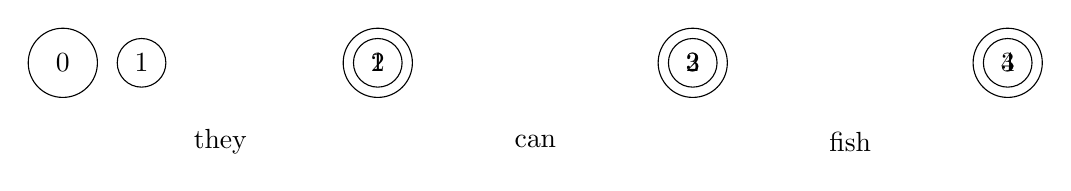
\begin{tikzpicture}[shorten >=2pt,auto,node distance=4cm]
      \node[state] (q1) {0};
      \node[state] (q2) [right of=q1] {1};
      \node[state] (q3) [right of=q2] {2};
      \node[state] (q4) [right of=q3] {3};
	  \node[draw,shape=circle] (a) at (1,0) {1};
	  \node[draw,shape=circle] (b) at (4,0) {2};
	  \node[draw,shape=circle] (c) at (8,0) {3};
	  \node[draw,shape=circle] (d) at (12,0) {4};
      
      \draw (2,-1) node (A) {they};
      \draw (6,-1) node  (B) {can};
      \draw (10,-1) node  (C) {fish};
\end{tikzpicture}
\\
Initialisiert wird mit einer leeren Menge von Kanten zwischen den bekannten Knoten. Der Algorithmus terminiert, wenn eine Kante zwischen Anfangs- und Endknoten gefunden wurde. Dies bedeutet, dass alle dazwischen liegenden Teilregeln ebenfalls gefunden wurden; der Suchbaum ist dann vollständig. Nach dem Durchlauf liegen dann alle möglichen Kanten, das heißt alle Teil- und Gesamtdeutungen des Satzes vor. Begonnen wird mit mit den ersten Knoten; diese werden dann mittels Kanten direkt nach den Regeln der Grammatik verbunden und nach und nach kommen weitere Kanten bis zum n-ten Wort hinzu. Wenn mehrere Kanten von erstem zu letztem Wort existieren, deutet dies dann auf eine Mehrdeutigkeit hin, da die Kanten dann verschiedene Produktionsregeln enthalten. Der Algorithmus sieht dann wie folgt aus:
\begin{enumerate} \tt
\item 
ChartParse: \\
for each Wort $w_{0-n}$ im Satz, sei \textit{from} der linke \\
und \textit{to} der rechte Knoten und daughters ds ein w \\
\hspace*{.2cm} for each möglichen Lexikoneintrag der Kategorie cat von w \\
\hspace*{.4cm} neueKante \textit{from,to,cat,ds} \\
output alle aufgespannten Kanten von $w_{0}$ nach $w_{n}$ \\ \rm(gesamter Text wird abgedeckt und mother ist S)\tt
\item 
neueKante: \textit{from,to,cat,daughters} \\
Neue Kante einzeichnen: \textit{id,from,to,cat,ds} \\
for each Regel linkeSeite -> $r_{1}-r_{n}$ einer cat aus der Grammatik \\
\hspace*{.2cm} Finde zusammenhängende Menge von Kanten \\
\hspace*{.2cm} $[id_{1},from_{1},to_{1},cat_{1},ds]$ bis $[id_{n-1},from_{n-1},from,cat_{n-1},ds_{n-1}]$ 

\rm(so einzeichnen, dass die Kante jeweils  eine bekannte Regel \\
zur Verbindung zwischen zwei Knoten enthält, also $to_{1}=from_{2}$ usw.)\tt \\
\hspace*{.2cm} For each Menge von Kanten, neueKante $from_{1},to,linkeSeite,id_{1}-id$ \rm(also alle Kanten weiter unterteilen)
\end{enumerate}
Bei Eingabe des Beispielsatzes würde die Ergebnistabelle aus \cite{cop04} folgende Kanten als Einträge beinhalten:

\begin{table}
\tt
\begin{tabular}{lllll}
$id$ & $knoten_{links}$ & $knoten_{rechts}$ & $mother$ & $daughters$ \\
1    & 0                & 1                 & NP       & (they)      \\
2    & 1                & 2                 & V        & (can)       \\
3    & 1                & 2                 & VP       & (2)         \\
4    & 0                & 2                 & S        & (1 3)       \\
5    & 2                & 3                 & V        & (fish)      \\
6    & 2                & 3                 & VP       & (5)         \\
7    & 1                & 3                 & VP       & (2 6)       \\
8    & 0                & 3                 & S        & (1 7)       \\
9    & 2                & 3                 & NP       & (fish)      \\
10   & 1                & 3                 & VP       & (2 9)       \\
11   & 0                & 3                 & S        & (1 10)     
\end{tabular}
\rm
\caption{Parsing-Tabelle gemäß Grammatikregeln aus \cite{cop04}}

Wie sich nun erkennen lässt, lässt sich anhand der mit S beginnenden Einträge aus der Tabelle der Satz generieren, indem nacheinander die Produktionsregeln aus jeder Zeile angewendet werden. Es lässt sich jede mögliche Deutung ablesen, die die Grammatik zulässt. Der Algorithmus gibt als Ergebnis also alle möglichen Parsbäume in der Tabelle an. Das Ergebnis kann wie folgt visualisiert werden (Ein schrittweises Beispiel findet sich in der Arbeit von Ann Copestake in Kapitel 4.8):

Wie sich nun erkennen lässt, lässt sich anhand der mit S beginnenden Einträge aus der Tabelle der Satz generieren, indem nacheinander die Produktionsregeln aus jder Zeile angewendet werden. Es lässt sich jede mögliche Deutung ablesen, die die Grammatik zulässt. Der Algorithmus gibt als Ergebnis also alles möglichen Parsbäume in der Tabelle an. Das Ergebnis kann wie folgt visualisiert werden (Ein schrittweises Beispiel findet sich in der Arbeit von Ann Copestake in Kapitel 4.8):

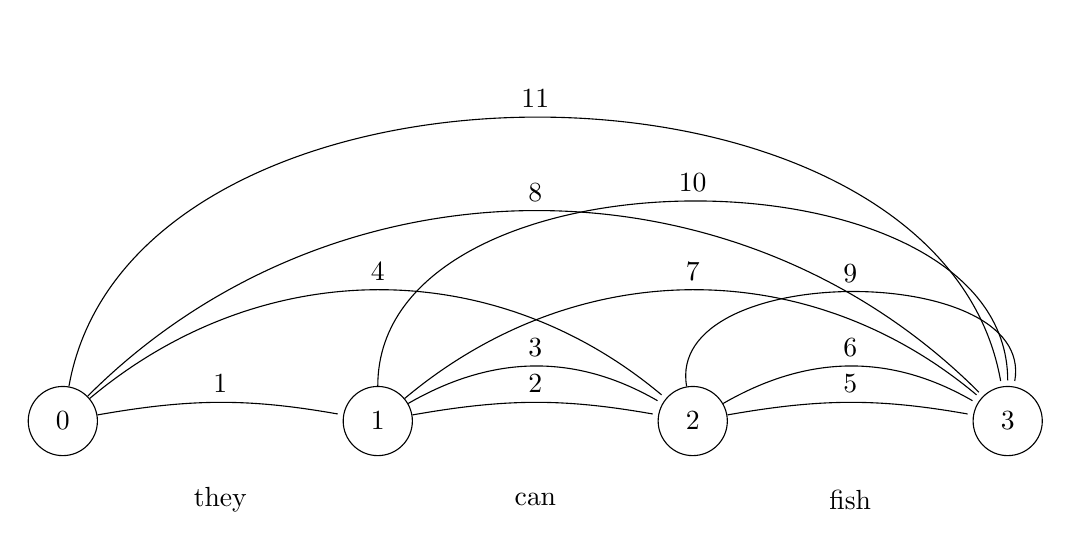
\begin{tikzpicture} [shorten >=2pt,auto,node distance=4cm]
      \node[state] (q1) {0};
      \node[state] (q2) [right of=q1] {1};
      \node[state] (q3) [right of=q2] {2};
      \node[state] (q4) [right of=q3] {3};
      
      \draw (2,-1) node (A) {they};
      \draw (6,-1) node  (B) {can};
      \draw (10,-1) node  (C) {fish};
      
      
      \draw (q1) to[bend left=10] node[auto] {1}(q2);
      \draw (q2) to[bend left=10] node[auto] {2}(q3);
      \draw (q2) to[bend left=30] node[auto] {3}(q3);
      \draw (q1) to[bend left=40] node[auto] {4}(q3);
      \draw (q3) to[bend left=10] node[auto] {5}(q4);
      \draw (q3) to[bend left=30] node[auto] {6}(q4);
      \draw (q2) to[bend left=40] node[auto] {7}(q4);
      \draw (q1) to[bend left=45] node[auto] {8}(q4);
      \draw (q3) to[bend left=100] node[auto] {9}(q4);
      \draw (q2) to[bend left=90] node[auto] {10}(q4);\\
      \draw (q1) to[bend left=80] node[auto] {11}(q4);
\end{tikzpicture}
\end{table}

\subsubsection{Mängel kontextfreier Grammatiken}
Die Umsetzung der Modellierung von Sprache auf Basis kontextfreier Grammatiken ist mit einigen Problemem verbunden. Zunächst scheint es vorteilhaft, wenn durch die Rekursion alle möglichen Teildeutungen erfasst werden; davon sind jedoch nicht alle sinnvoll und viele redundant, weil sinnlos. Es fällt auf, dass durch die Zerlegung in Teildeutungen durch Anwendung aller möglichen Regeln aus der Grammatik prinzipiell exponentiell viele Deutungen entstehen könnten. Teilweise würden auch grammatikalisch falsche Sätze akzeptiert, wenn nicht jeder Numerus, Kasus etc. eines Wortes als Terminalsymbol in der Menge an Produktionsregeln repräsentiert wird. In der obigen einfachen Grammatik wird \textit{"they fish"} genau so wie \textit{"it fish"} akzeptiert. 

Ferner werden Zusammenhänge aus Wörtern, die sich inhaltlich aufeinander beziehen, nicht abgebildet und nicht aus dem Kontext erfasst. Manche Verben erscheinen etwa ohne Berücksichtigung des Satzobjektes für den Menschen eher sinnlos, \textit{"Felix erwartet"} scheint unvollständig, die richtige Deutung von Zusammenhängen \textit{"Felix erwartet Aaron"} schließt den Kontext des Teilsatzes ein.

Eine Möglichkeit zur Lösung wird in Abschnitt 2.6 und 2.7 behandelt, indem der Konsens einer Formulierung ebenso wie Ansätze der Semantik bei der Deutung berücksichtigt werden. Dies ist mittels einfacher Produktionsregeln nicht möglich.

\subsection{Parsen mit constraint-basierten Grammatiken}
Wie zuvor an verschiedenen Beispielen demonstriert wurde, weisen die kontextfreien Grammatiken beim Parsen und Generieren einige schwächen auf. Daher wird im folgenden Abschnitt ein neuer, komplexerer Ansatz vorgestellt um sich mit den gleichen Problemen zu befassen. Kontextfreie Grammatiken können als constraint-basiert interpretiert werden, diese Bezeichnung wird jedoch üblicherweise für mächtigere Grammatiken verwendet. Constraint-basierte Grammatiken sind in NLP weit verbreitet und werden mit sogenannten feature-structures (Eigenschaftsstrukturen) dargestellt, daher auch oft feature-structure (FS) Grammatik genannt. Im folgenden Abschnitt soll die Umsetzung solch einer Grammatik durch feature-structures demonstriert werden.

%\subsubsection{Beispiel zu einfacher FS Grammatik}

FSs sind Graphen, welche große Ähnlichkeit zu Baumstrukturen aufweisen. Sie haben genau eine Wurzel und sind von dieser aus gerichtet. Ein Knoten kann keinen, einen oder mehrere Kindesknoten besitzen. Endknoten, also Knoten mit dem Ausgangsgrad 0 verfügen über Werte und Kanten sind mit Eigenschaften versehen. Ein Weg entlang von Eigenschaften wird als Pfad bezeichnet. Eigenschaften sind entweder atomar oder zusammengesetzt, abhängig davon ob sie auf einen Endknoten oder auf einen weiteren nicht-Endknoten zeigen. In dem folgenden, dem Paper entnommenen Beispiel ist eine FS abgebildet, die sich in zwei Eigenschaften, \textit{"CAT"} für die Wortkategorie und \textit{"AGR"} für agreement (Stimmigkeit), teilt, welche jeweils auf die Endknoten mit den Werten \textit{"noun"} (für Nomen) und \textit{"sg"} (für Singular) zeigen. Die Eigenschaften \textit{"CAT"} und \textit{"AGR"} sind also atomar.

\begin{center}
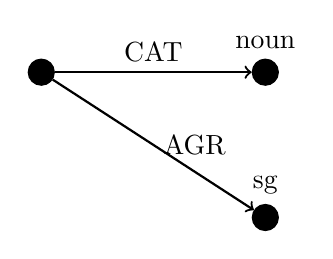
\begin{tikzpicture}
\node[draw,shape=circle,fill=black] (a) at (0,0) {};
\node[draw,shape=circle,fill=black,label=above:noun] [right = 2.5cm of a] (b) {};
\node[draw,shape=circle,fill=black,label=above:sg] [below = 1.5cm of b] (c) {};

\draw[thick, ->] (a) to node[midway, above] {CAT} (b);
\draw[thick, ->] (a) to node[midway, above, right] {AGR} (c);
\end{tikzpicture}
\end{center}

Fügt man wie in der nächsten Abbildung vor der Wurzel eine weitere Eigenschaft \textit{"Head"} hinzu, so ist diese zusammengesetzt, da sie auf einen nicht-Endknoten zeigt. Dieser wird wiederum in die beiden Eigenschaften \textit{"CAT"} und \textit{"AGR"} aufgeteilt. 

\begin{center}
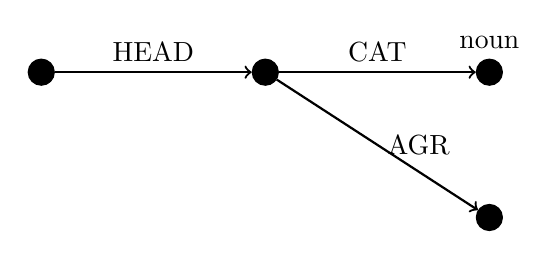
\begin{tikzpicture}

\node[draw,shape=circle,fill=black] (a) at (0,0) {};
\node[draw,shape=circle,fill=black,label=above:noun,right = 2.5cm of a] (b) {};
\node[draw,shape=circle,fill=black,below = 1.5cm of b] (c) {};
\node[draw,shape=circle,fill=black,left = 2.5cm of a] (d) {}; 

\draw[thick, ->] (a) to node[midway, above] {CAT} (b);
\draw[thick, ->] (a) to node[midway, above, right] {AGR} (c);
\draw[thick, ->] (d) to node[midway, above] {HEAD} (a);
\end{tikzpicture}
\end{center}

Solche Strukturen lassen sich am besten als attribute-value matrices (Attribut-Wert Matrizen, AVMs) aufschreiben was dann wie folgt aussieht:



In FSs ist es möglich, dass mehrere Pfade zu dem gleichen Endknoten erreichen, was als Eintrittsinvarianz bezeichnet wird. Sollte dies bei einem Endknoten zutreffen, so wird dessen Wert durch einen eingeklammerten Integer dargestellt. Der numerische Wert dieses Integers ist irrelevant, da er als Platzhalter für einen tatsächlichen grammatikalischen Wert verwendet wird. Dabei ist zu beachten, dass dann für gleiche Integer auch der gleiche Wert eingesetzt wird, was jedoch erst in einem späteren Abschnitt genauer beschrieben wird. 



\subsection{Lexikalische Semantiken und kontextbasierte Deutungen}

\newpage

\begin{thebibliography}{5}
\bibitem[COP04]{cop04}Ann Copestake, University Of Cambridge, "Natural Language Processing", 2004
\bibitem[CLW7]{clw7}University Centre for Computer Corpus Research on Language, Lancaster University, "CLAWS part-of-speech tagger for English", http://ucrel.lancs.ac.uk/claws/, abgerufen am 19.08.2018 16.43 Uhr
\bibitem[CHO57]{cho57} Noam Chomsky, "Syntactic Structures", Mouton \& Co., Feb. 1957

\end{thebibliography}
\end{document}
